% flashcards-title: Adding a negative number as a leftward jump on the number line
% flashcards-desc: A horizontal number line with arrowheads on both ends and evenly spaced marks; the marks at 0 and 3 are labeled. A round dot sits on the mark at 3, and a curved arrow labeled plus negative five jumps five marks leftward from the dot, landing on a mark labeled with a question mark.
\documentclass[tikz]{standalone}
\usetikzlibrary{arrows.meta,patterns}

\definecolor{qraNavy}{HTML}{17324D}
\definecolor{qraBlue}{HTML}{2B6CB0}
\definecolor{qraGold}{HTML}{B7791F}
\definecolor{qraPale}{HTML}{EAF2F8}
\definecolor{qraGray}{HTML}{5C6773}

\tikzset{
  qra axis/.style={draw=qraNavy, line width=1.2pt},
  qra tick/.style={draw=qraNavy, line width=1pt},
  qra guide/.style={draw=qraGray, densely dashed, line width=0.8pt},
  qra counter/.style={circle, draw=qraNavy, fill=qraPale, line width=0.9pt, minimum size=7mm, inner sep=0pt},
  qra label/.style={font=\sffamily\bfseries, text=qraNavy},
  qra small label/.style={font=\sffamily, text=qraNavy},
}

\begin{document}
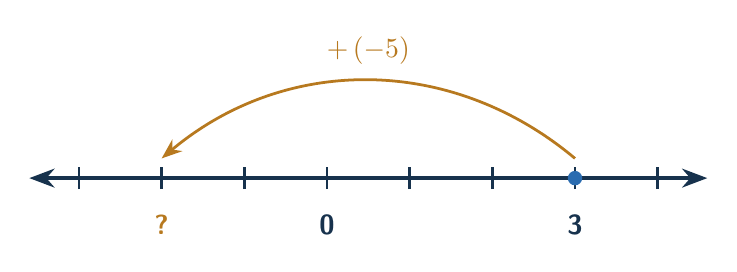
\begin{tikzpicture}[x=1.05cm]
  % Axis with arrowheads both ways
  \draw[qra axis, {Stealth[length=3.2mm]}-{Stealth[length=3.2mm]}] (-3.6,0) -- (4.6,0);

  % Ticks -3..4; labels only on 0 and 3
  \foreach \n in {-3,...,4} {
    \draw[qra tick] (\n,-0.14) -- (\n,0.14);
  }
  \node[qra label, below=6pt] at (0,-0.14) {0};
  \node[qra label, below=6pt] at (3,-0.14) {3};
  \node[qra label, text=qraGold, below=6pt] at (-2,-0.14) {?};

  % Start dot at 3
  \fill[qraBlue] (3,0) circle (2.6pt);

  % Leftward jump of five marks, arcing above the line
  \draw[qra tick, draw=qraGold, -{Stealth[length=2.6mm]}]
    (3,0.25) to[bend right=40] node[qra small label, above=2pt, text=qraGold] {$+\,(-5)$} (-2,0.25);
\end{tikzpicture}
\end{document}
